\documentclass[12pt]{article}
\usepackage[T2A]{fontenc}
\usepackage[utf8]{inputenc}
\usepackage{multirow}
\usepackage{caption}
\usepackage{subcaption}
\usepackage{amsmath}
\usepackage{changepage}
\usepackage{graphicx}
\usepackage{float}
\usepackage[english,russian]{babel}
\usepackage{amsmath, amsfonts, amssymb, amsthm, mathtools}
\usepackage{xcolor}
\usepackage{array}
\usepackage{hyperref}
\usepackage[top = 1.5cm, left = 1.5 cm, right = 1.5 cm, bottom = 3 cm]{geometry}
\graphicspath{ {./images/} }
 
\title{Измерение коэффициента диффузии гелия при атмосферном давлении.}
\author{Шахматов Андрей, Б02-304}
\date{\today}
  
\begin{document}
\begin{titlepage}
    \begin{center}
        {\large МОСКОВСКИЙ ФИЗИКО-ТЕХНИЧЕСКИЙ ИНСТИТУТ (НАЦИОНАЛЬНЫЙ ИССЛЕДОВАТЕЛЬСКИЙ УНИВЕРСИТЕТ)}
    \end{center}
    \begin{center}
        {\large Физтех-школа физики и исследований им. Ландау}
    \end{center}
    
    
    \vspace{3cm}
    {\huge
        \begin{center}
            \textbf{Измерение коэффициента диффузии гелия при атмосферном давлении.}
        \end{center}
    }
    \vspace{2cm}
    \begin{flushright}
        {\LARGE Автор:\\ Шахматов Андрей Юрьевич \\
            \vspace{0.2cm}
            Б02-304}
    \end{flushright}
    \vspace{7 cm}
    \begin{center}
        Долгопрудный 2024
    \end{center}
\end{titlepage}

% \maketitle

\begin{abstract}
    Исследована зависимость коэффициента диффузии гелия в зависимости от давления. Для этого 
    исследована зависимость концентрации гелия от времени в процессе диффузии гелий-воздух. 
    Найден коэффициент диффузии гелия при атмосферном давлении. Полученное значение совпало с 
    табличным значением коэффициента диффузии гелия.       
\end{abstract}

\tableofcontents

\section{Введение}
Цель настоящей работы заключалась в исследовании протекания процесса диффузии на примере гелия, а также 
опредления его коэффициента диффузии в зависимости от давления.

\section{Методика}
\section*{Теоретическое введение}
Рассмотрим процесс выравнивания концентрации. Пусть концентрации одного из компонентов смеси в сосудах $V_1$ и $V_2$ равны $n_1$ и
$n_2$. Плотность диффузионного потока любого компонента (т. е. количество вещества, проходящее в единицу времени через единичную поверхность) определяется законом Фика:
$$j=-D\frac{\partial n}{\partial x},$$ где $D$ — коэффициент взаимной диффузии газов, а $j$ - плотность потока частиц.

В нашем случае ввиду того что, а) объем соединительной трубки мал по сравнению с объемами сосудов, б) концентрацию газов внутри каждого сосуда можно считать постоянной по всему объему. Диффузионный поток в любом сечении трубки одинаков. Поэтому, $$J=-DS\frac{n_1-n_2}{l}.$$

Обозначим через $\Delta n_1$ и $\Delta n_2$ изменения концентрации в объемах
$V_1$ и $V_2$ за время $\Delta t$. Тогда $V_1 \Delta n_1$ равно изменению количества компонента в объеме $V_1$, а $V_2 \Delta n_2$ — изменению количества этого компонента в $V_2$. Из закона сохранения вещества следует, что $V_1n_1+V_2n_2 = const$, откуда $V_1 \Delta n_1 = -V_2\Delta n_2.$ Эти изменения происходят вследствие диффузии, поэтому: $$V_1\Delta n_1=-V_2\Delta n_2.$$

С другой стороны $V_1\Delta n_1=J\Delta t$ и $V_1\frac{dn_1}{dt}=-DS\frac{n_1-n_2}{l}.$ Аналогично $V_2\frac{dn_2}{dt}=DS\frac{n_1-n_2}{l}$

Тогда $$\frac{d(n_1-n_2)}{dt}=-\frac{n_1-n_2}{l} \frac{V_1+V_2}{V_1V_2}.$$

Проинтегрируем и получим, что $$n_1-n_2=(n_1-n_2)_0 e^{-t/\tau},$$ где $(n_1-
    n_2)_0$ — разность концентраций в начальный момент времени, $$\tau=\frac{V_1V_2}{V_1+V_2}\frac{L}{SD}.$$

В нашей установке объёмы сосудов примерно равны $V = V_1 = V_2$. 
Для измерения концентраций в данной установке применяются датчики теплопроводности $Д_1$, $Д_2$ (см. рис. 1) используется зависимость теплопроводности газовой смеси от ее состава.
Для измерения разности концентраций газов используется мостовая схема (рис. 1). Здесь $Д_1$ и $Д_2$ — датчики теплопроводности, расположенные в сосудах $V_1$ и $V_2$. Сопротивления $R_1, R_2$ и $R$ служат для установки прибора на нуль (балансировка моста). В одну из диагоналей моста включен гальванометр, к другой подключается небольшое постоянное напряжение. Мост балансируется при заполнении сосудов (и датчиков) одной и той же смесью.

При заполнении сосудов смесями различного состава возникает «разбаланc» моста. При незначительном различии в составах смесей показания гальванометра, подсоединённого к диагонали моста, будут пропорциональны разности концентраций примеси. В процессе диффузии
разность концентраций убывает по экспоненте, и значит по тому же закону изменяются во времени показания гальванометра $$U=U_0 \exp(-t/\tau).$$
\section*{Эксперементальная установка}
Схема установки изображена на рис. 1. Там же показана схема электрических соединений и конструкция многоходового крана $K_6$

\begin{figure}[h]
    \center{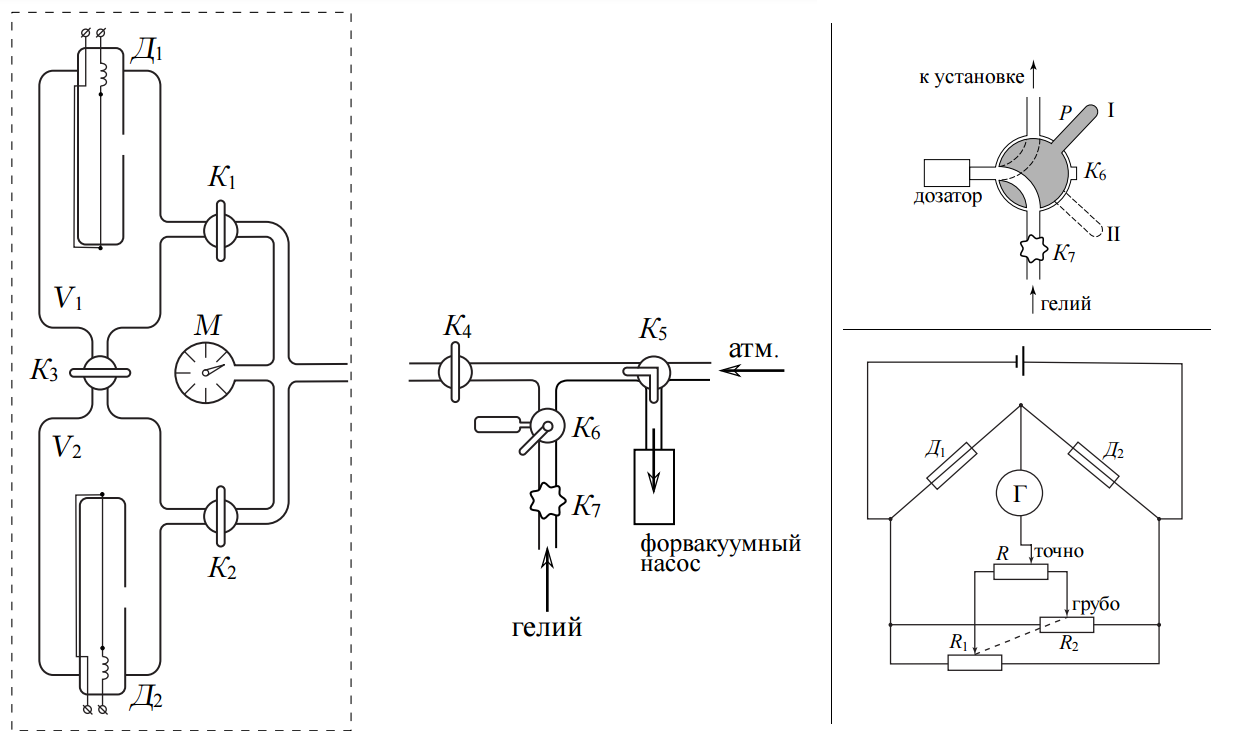
\includegraphics[scale=0.6]{lab_2_2_1_ust.png}}
    \caption{Схема экспериментальной установки.}
\end{figure}
Установка состоит из двух сосудов $V_1$ и $V_2$ соединенных краном $К_3$, форвакуумного насоса Ф.Н. с выключателем $Т$, манометра $M$ и системы напуска гелия, включающей в себя краны $К_6$ и $К_7$. Кран $К_5$ позволяет соединять форвакуумный насос либо с установкой, либо с атмосферой. Между форвакуумным насосом и краном $К_5$ вставлен предохранительный баллон П.Б., защищающий кран $К_5$ и установку при неправильной эксплуатации ее от попадания форвакуумного масла из насоса Ф.Н. Сосуды $V_1$ и $V_2$ и порознь и вместе можно соединять как с системой напуска гелия, так и с форвакуумным насосом. Для этого служат краны $К_1$, $К_2$, $К_4$ и $К_5$. Манометр  $M$
регистрирует давление газа, до которого заполняют тот или другой
сосуды.

Для сохранения гелия, а также для уменьшения неконтролированного попадания гелия в установку (по протечкам в кране $К_6$) между
трубопроводом подачи гелия и краном $К_6$ поставлен металлический
кран $К_7$. Его открывают только на время непосредственного заполнения установки гелием. Все остальное время он закрыт.

В силу того, что в сосуд требуется подавать малое давление гелия,
между кранами $К_7$ и $К_4$ стоит кран $К_6$, снабженный дозатором. Дозатор - это маленький объем, который заполняют до давления гелия в трубопроводе, а затем уже эту порцию гелия с помощью крана $К_6$ впускают в установку.

Описание схемы электрического соединения. $Д_1$ и $Д_2$ — сопротивления проволок датчиков парциального давления, которые составляют одно плечо моста. Второе плечо моста составляют сопро- тивления $r_1$, $R_1$ и $r_2$, $R_2$. $r_1 \ll R_1$, $r_2 \ll R_2$, $R_1$ и $R_2$ спаренные, их подвижные контакты находятся на общей оси. Оба они исполь- зуются для грубой регулировки моста. Точная балансировка моста выполняется потенциометром R. Последовательно с гальванометром $Г$, стоящим в диагонали моста, поставлен магазин сопротивлений $MR$. Когда мост балансируют, магазин сопротивлений выводят на ноль. В процессе же составления рабочей смеси в сосудах $V_1$ и $V_2$ мост разбалансирован. Чтобы не сжечь при этом гальванометр, магазин $MR$ ставят на максимальное сопротивление.


\section{Результаты и их обсуждение}
Измерена зависимость концентрации гелия от времени при различных начальных давлениях $P$. Соотношение 
давлений и номеров эксперимента представленно в таблице \ref{tab:1}. Построим соответствующие зависимости 
(Рис. \ref{fig:Vt}).   

\begin{figure}[H]
    \centering
    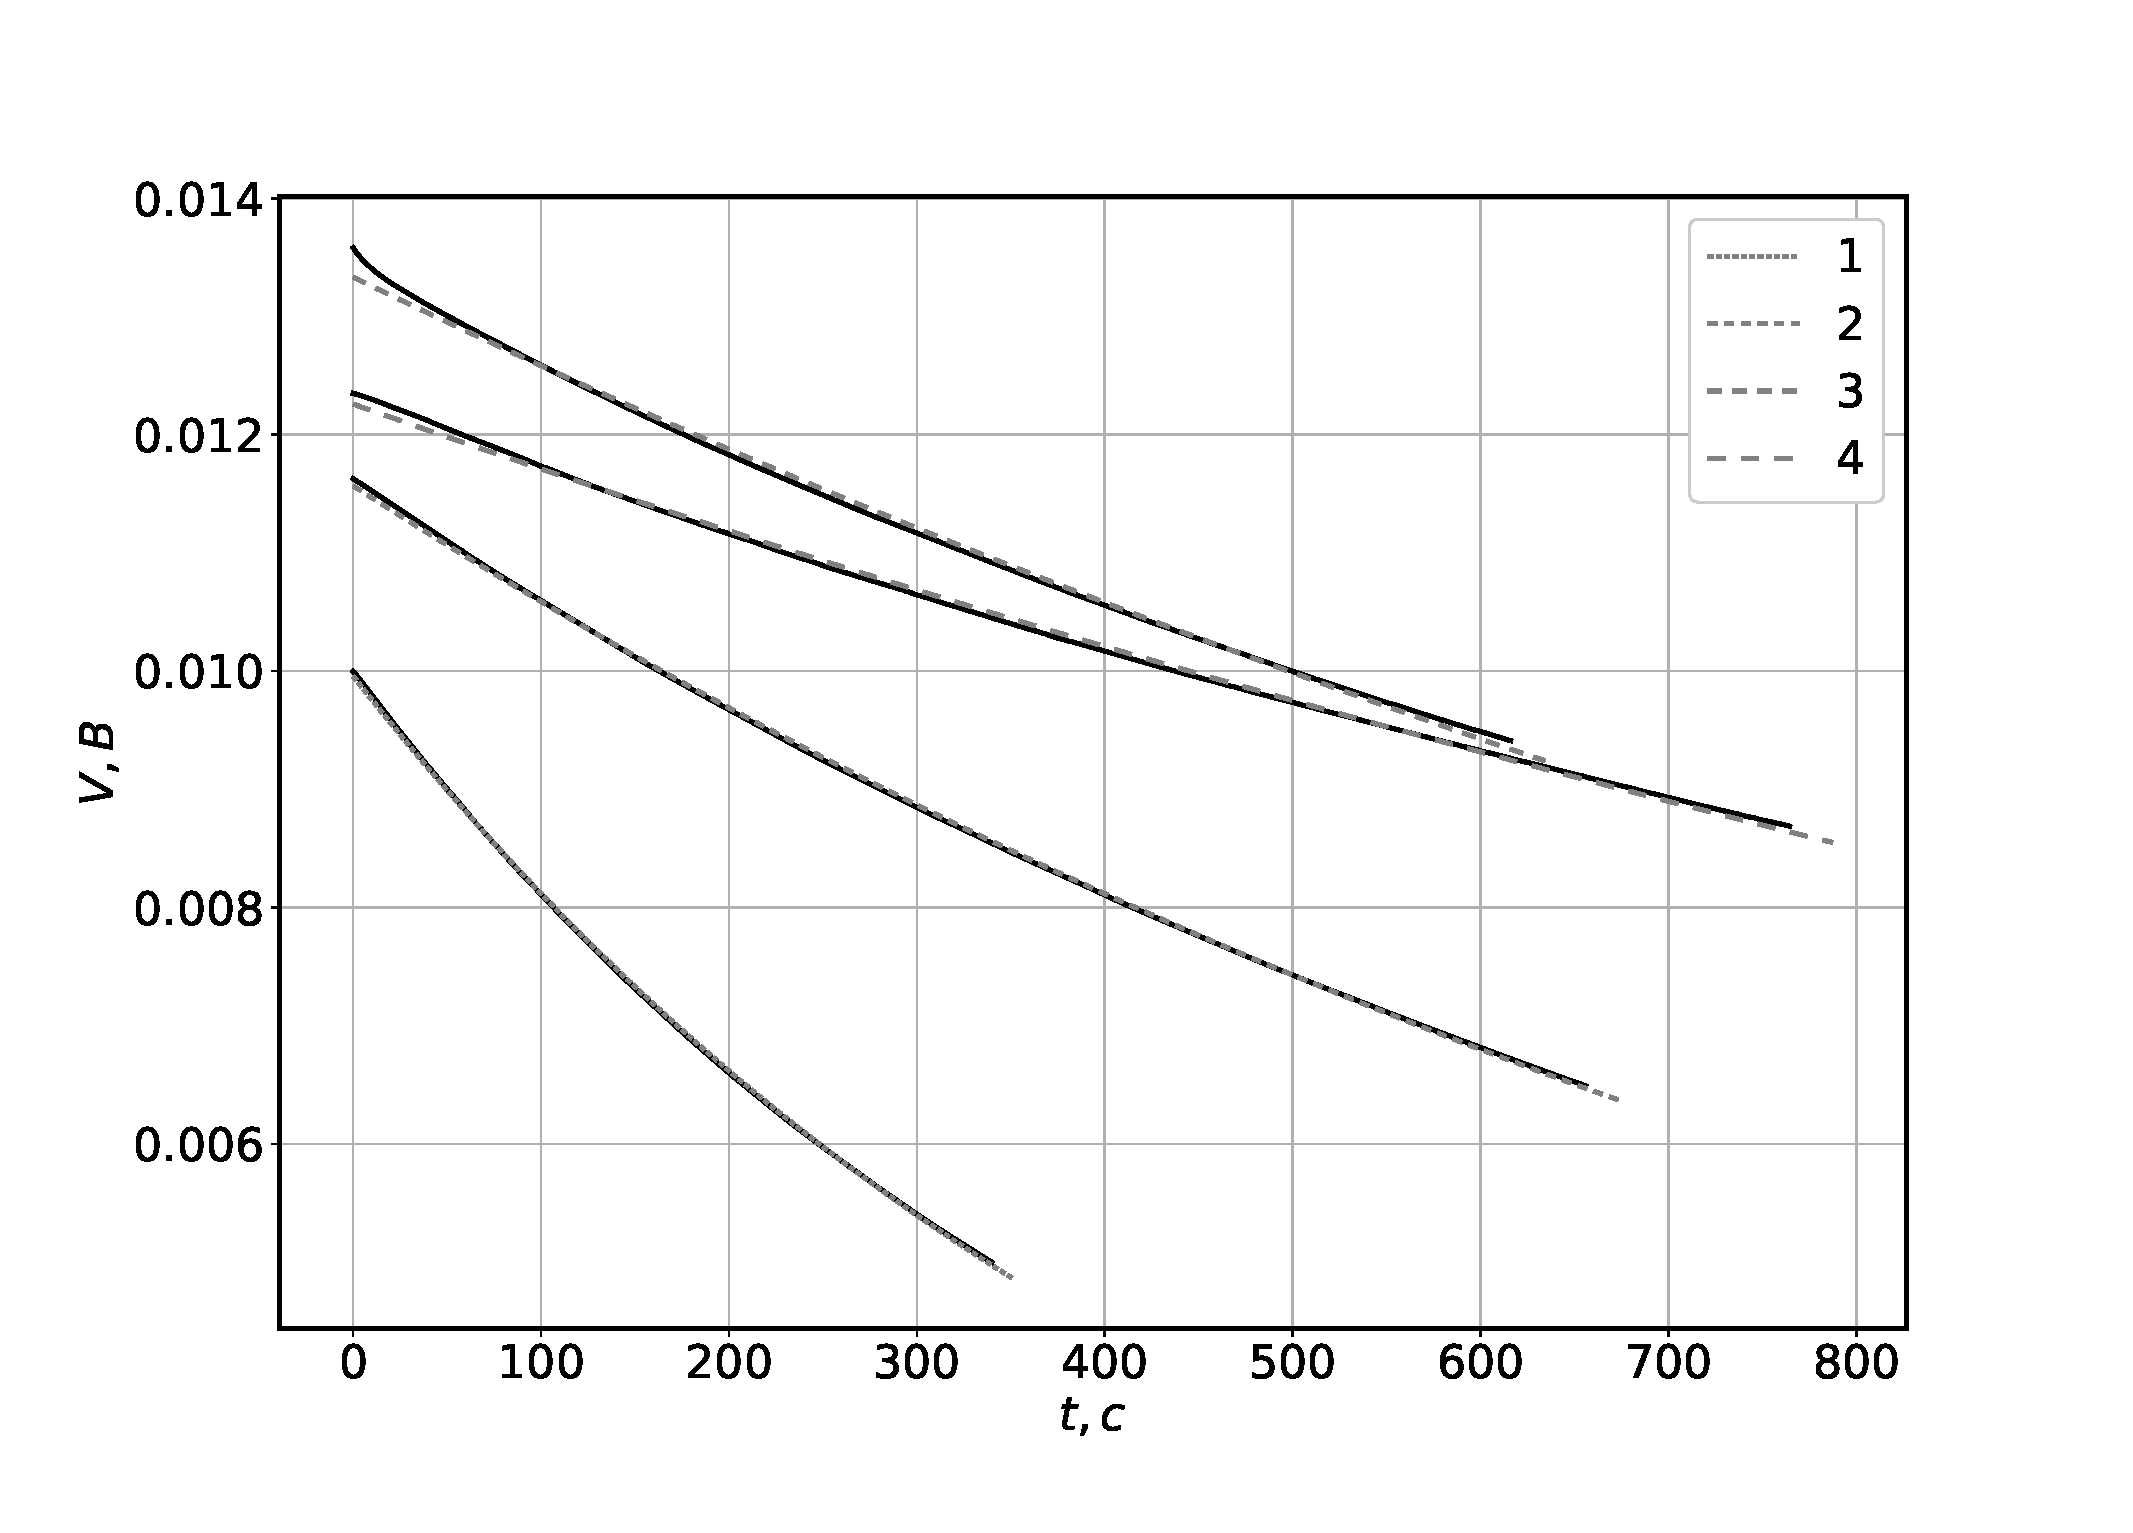
\includegraphics[width=0.8\textwidth]{Vt.eps}
    \caption{Зависимости разности напряжений на вольтметре $V$ в зависимости от времени проведения
        эксперимента. Цифрами обозначены эксперименты, проведённые при соответствующих давлениях представленных 
        в таблице \ref{tab:1}. Пунктирными линиями обозначены кривые, соответствующие экспоненциальному 
        затуханию.}
    \label{fig:Vt}
\end{figure}

Согласно теории, зависимости должны иметь вид $V = V_0 \exp -\frac{t}{\tau}$. Для 
проверки построим зависимости в логарифмическом масштабе $\ln V = \ln V_0 - \frac{t}{\tau}$ (Рис. \ref{fig:lnVt}).
Из рисунков видно, что все зависимости точно ложатся на прямые линии, потому можно считать теоретическую модель 
применимой. 

\begin{figure}[H]
    \centering
    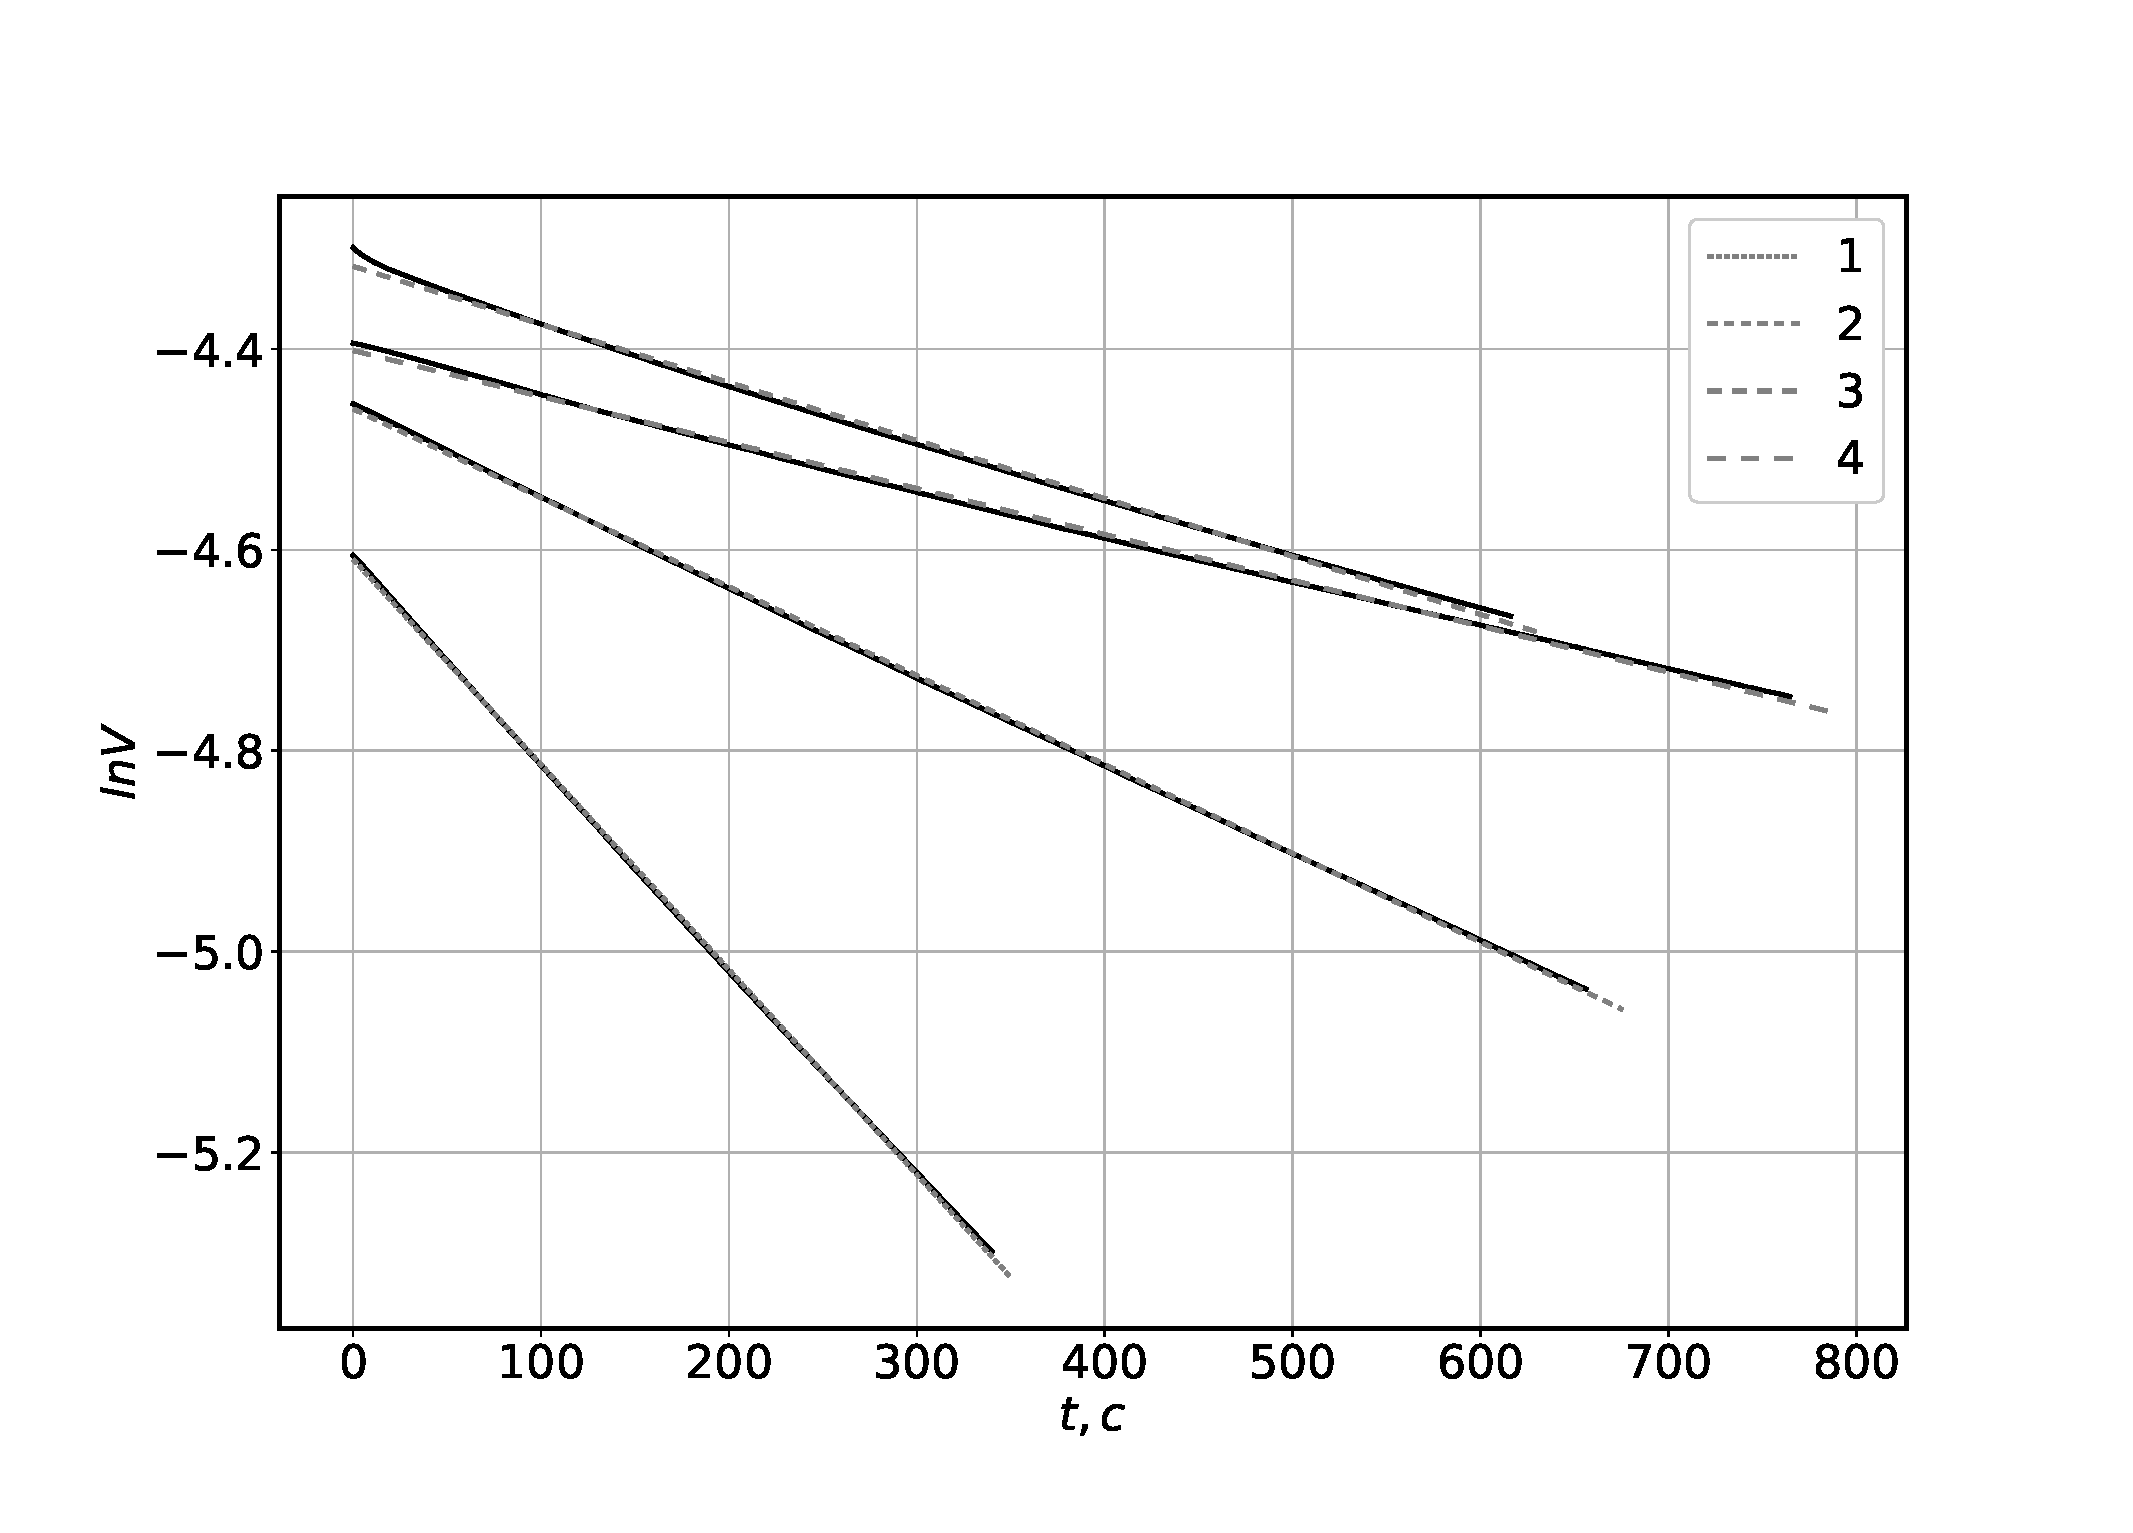
\includegraphics[width=0.8\textwidth]{lnVt.eps}
    \caption{Зависимости разности напряжений на вольтметре $V$ в зависимости от времени проведения
        эксперимента в логарифмическом масштабе. Цифрами обозначены эксперименты, проведённые при соответствующих давлениях представленных 
        в таблице \ref{tab:1}.}
    \label{fig:lnVt}
\end{figure}

Вычислены значения коэффициентов наклона $\frac{1}{\tau}$ и согласно формуле:
\[
    D = \frac{1}{2} \frac{L}{S \tau}
\]
вычислены коэффициенты диффузии гелия. Согласно теории коэффициент диффузии обратно пропорционально зависит от давления 
газа. Построим зависимости $D(\frac{1}{P})$ (Рис. \ref{fig:D2P}). Так как зависимость оказалась линейной 
возможно экстраполировать график к значению диффузии при атмосферном давлении $P_0 = 760 Торр$. Полученный 
коэффициент оказался равен $D_0 = &D_0&$ $\frac{\text{м}^2}{\text{с}}$.    

\begin{figure}[H]
    \centering
    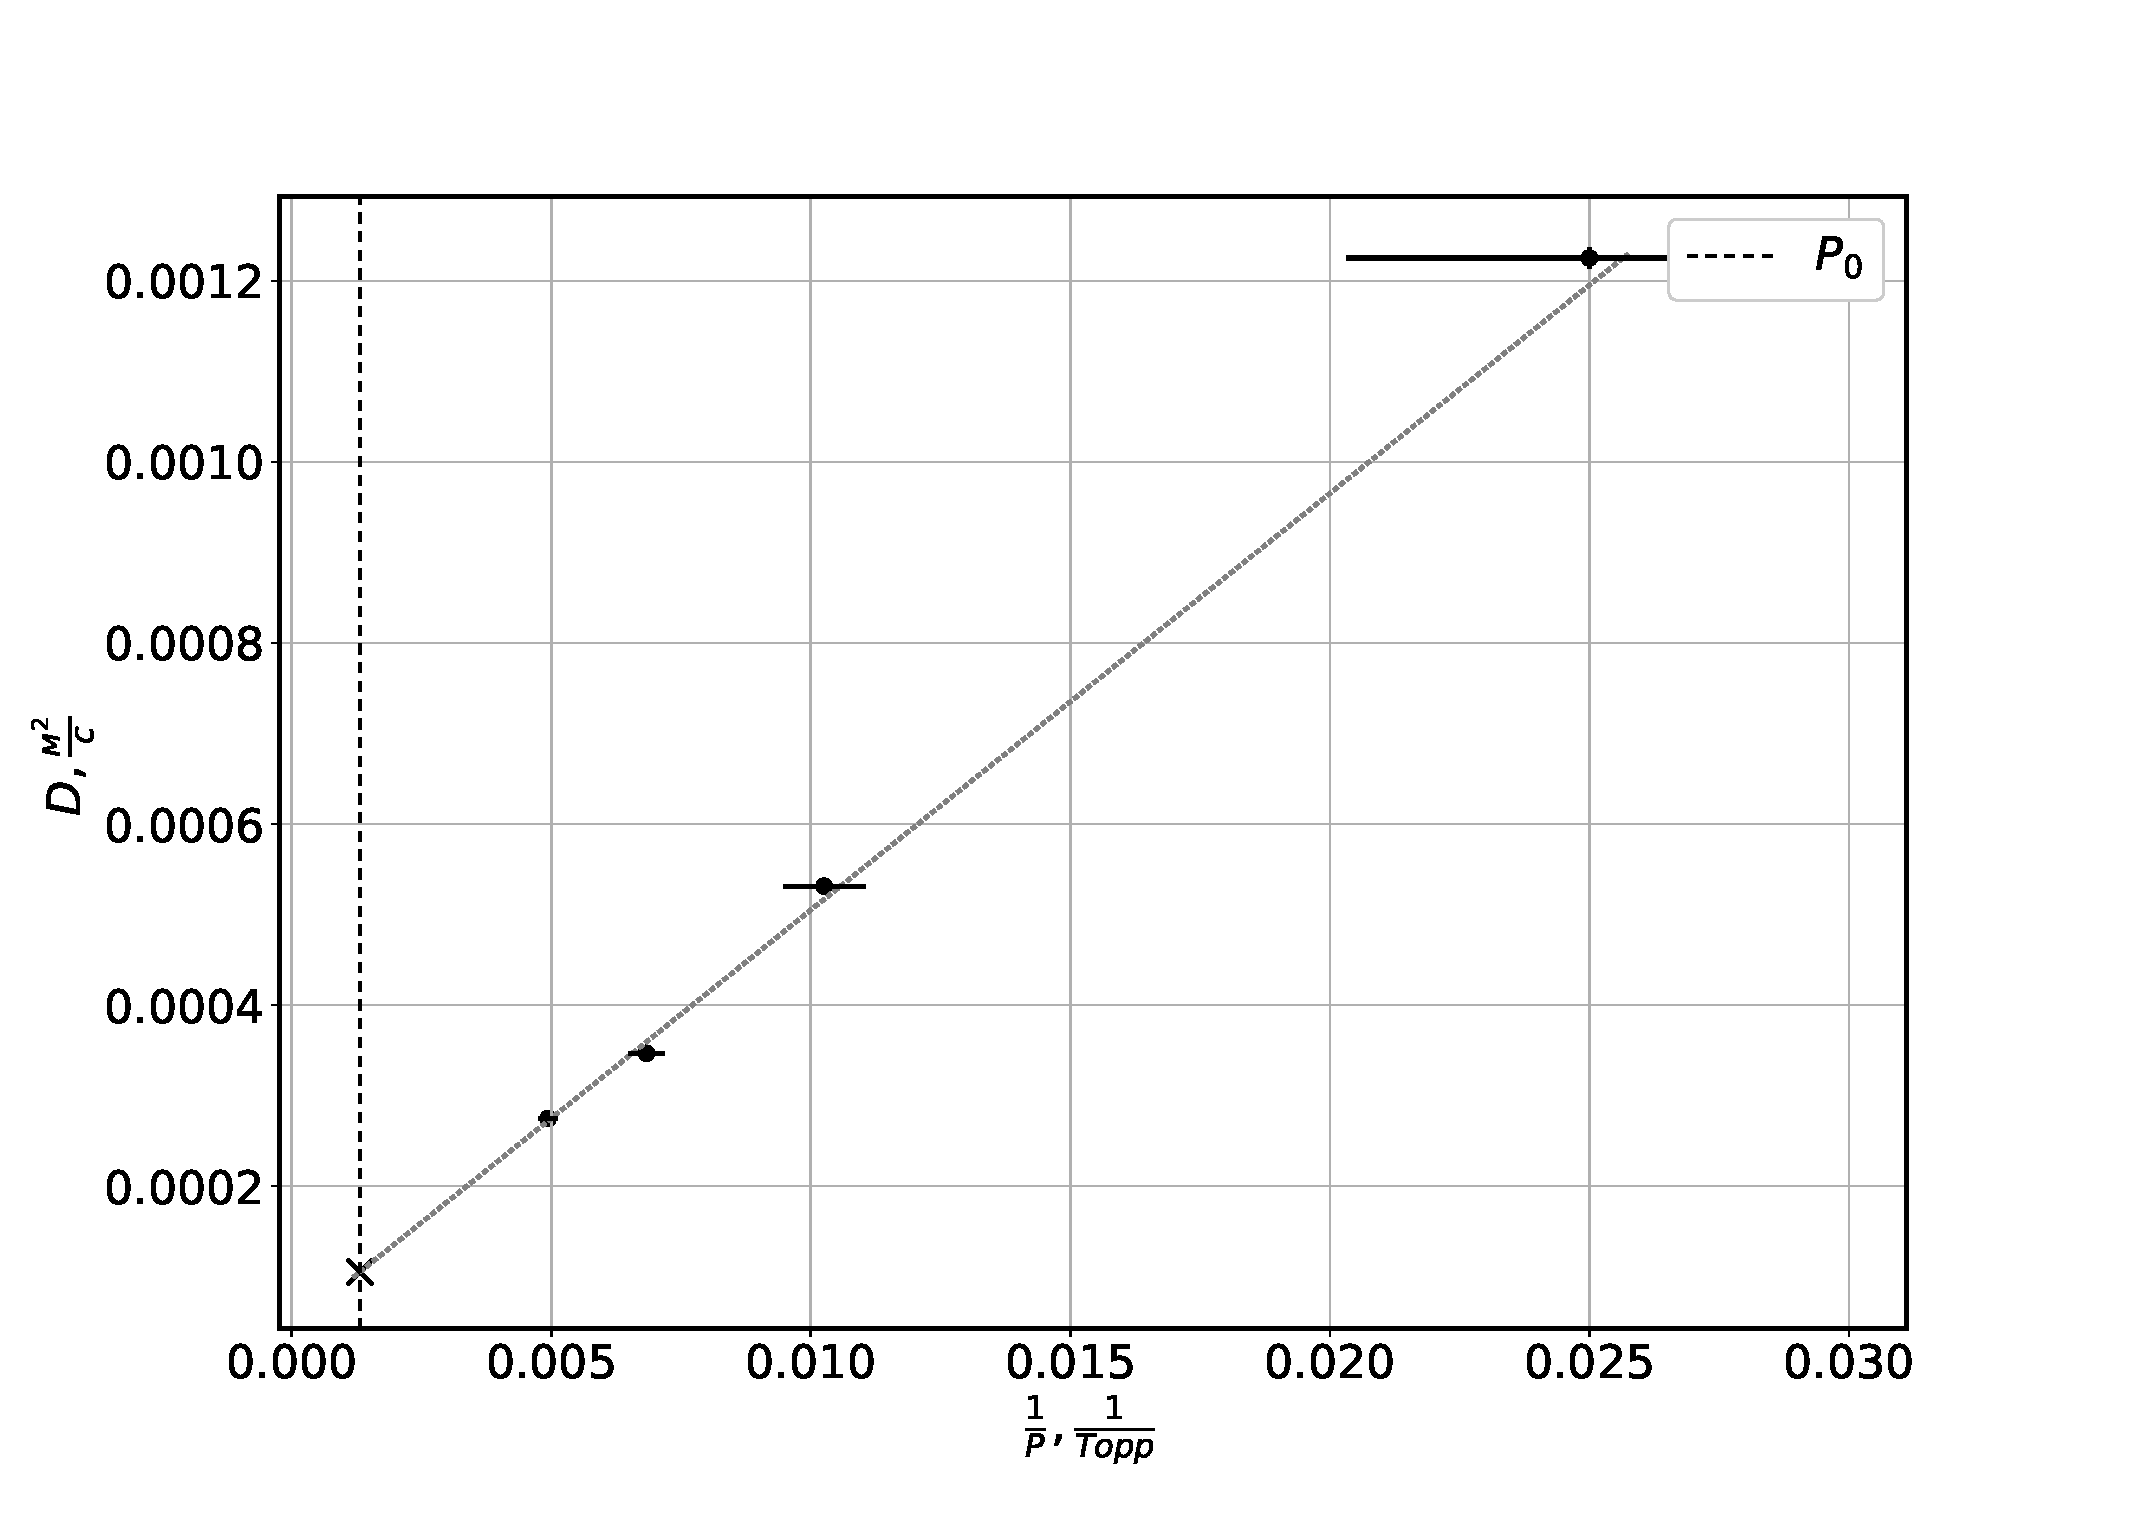
\includegraphics[width=0.8\textwidth]{D2P.eps}
    \caption{Зависимость коэффициента диффузии гелия $D$ в зависимости от давления $\frac{1}{P}$.}
    \label{fig:D2P}
\end{figure}

\section{Выводы}
Проведено измерение коэффициента диффузии гелия в зависимости от его давления. Определён вид 
зависимости коэффициент диффузии от давления. С помощью экстраполяции найден коэффициент диффузии гелия 
при одной атмосфере. Полученное значение совпало с табличным значением коэффициента диффузии гелия при 
атмосферном давлении.

\section{Использованная литература}
\begin{thebibliography}{9}
    \bibitem{LabBook}
    Лабораторный практикум по общей физике, Том 1, под редакцией А. Д. Гладуна
    \bibitem{Kirichenko}
    Н.А. Кириченко «Термодинамика, статистическая и молекулярная физика».
\end{thebibliography}

\section{Приложения}
\subsection{Параметры установки и погрешности приборов} \label{app_1}
Объём сосуда установки равен $V = &V&$ $\text{м}^3$, отношение длины участка диффузии к площади его сечения равно 
$\frac{L}{S} = &L2S&$ $\frac{1}{\text{м}}$.     
\subsection{Данные результатов измерений} \label{app_2}
\begin{table}[H]
    \centering
    \begin{tabular}{|r|r|}
        \hline
        $N$ & $P$, Па \\
        \hline
        1   & 40.0    \\
        2   & 97.5    \\
        3   & 146.3   \\
        4   & 202.5   \\
        \hline
    \end{tabular}
    
    \caption{Соотношение номера эксперимента $N$ и приготовленного давления в установке $P$.}
    \label{tab:1}
\end{table}
\end{document}